% !TeX root = ./slides-11.tex

\setcounter{section}{10}
\section{Interpretations for full QL}

\subsection{Interpretations and truth, revisited}

\begin{frame}
\frametitle{Interpretations}

\begin{itemize}[<+->]
\item Domain: collection of objects (not empty)
\item \emph{Referents} for each name (which object it names)
\item Properties of each object
  \begin{itemize}
  \item \emph{Extension} of each 1-place predicate symbol: which
  objects it applies to
  \end{itemize}
\item Relations of each pair of objects
\begin{itemize}
\item \emph{Extension} of each $2$-place predicate symbol: which pairs of
  objects standing in the relation
\item Extension of $=$ is all pairs $\langle\alpha, \alpha\rangle$.
\end{itemize}
\end{itemize}

\end{frame}

\begin{frame}
\frametitle{Extensions of predicates}

\begin{ekey}
\item[$Domain$] $1$, $2$, $3$
\item[$a$] $1$
\item[A\qr{x}{y}] $\langle 1, 1\rangle$, $\langle 1,2\rangle$, $\langle 1,3\rangle$, $\langle 2,3\rangle$
\end{ekey}
\usetikzlibrary{arrows}
\hfill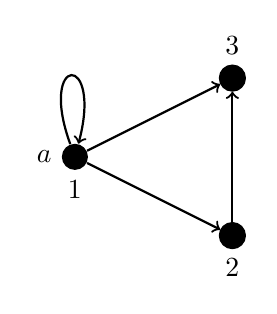
\begin{tikzpicture}
    \node[circle,fill,label={below:$1$},label={left:$a$}] (A) at (-1,0) {};
    \node[circle,fill,draw,label={below:$2$}] (B) at (1,-1) {};
    \node[circle,fill,draw,label={above:$3$}] (C) at (1,1) {};
    \draw[->,thick] (A) to[loop above,looseness=30,out=110] (A);
    \draw[->,thick] (A) -- (B);
    \draw[->,thick] (A) to (C);
    \draw[->,thick] (B) -- (C);
\end{tikzpicture}
\end{frame}

\begin{frame}
  \frametitle{Truth of sentences of QL}

  \begin{itemize}[<+->]
    \item Given an interpretation $I$ \dots
    \item An \emph{atomic sentence} is true iff the referents of the constants are in the extension of the predicate:
    \begin{itemize}
    \item $P\qv{a}$ is true iff referent $\alpha$ of $a$ is in extension of $P$
    \item $R\qr{a}{b}$ is true iff $\langle \alpha,\beta\rangle$ is in extension of $R$\\
    (where $\alpha$ is referent of $a$, $\beta$ is referent of $b$)
    \item $a=b$ true iff $a$ and $b$ are names for one and the the same object.
    \end{itemize}
    \item $\enot\metav{A}$ is true iff $\metav{A}$ is false
    \item $\metav{A} \eor \metav{B}$ is true iff at least one of $\metav{A}$, $\metav{B}$ is true
    \item $\metav{A} \eand \metav{B}$ is true iff both $\metav{A}$, $\metav{B}$ are true
    \item $\metav{A} \eif \metav{B}$ is true iff $\metav{A}$ is false or $\metav{B}$ is true
  \end{itemize}
\end{frame}

\begin{frame}
  \frametitle{Satisfaction of formulas}

  \begin{itemize}[<+->]
    \item Suppose $\metav{A}\qv{\metav{x}}$ has only the variable $\metav{x}$
    free.
    \item Object $\alpha$ in domain \emph{satisfies} $\metav{A}\qv{\metav{x}}$ iff $\metav{A}\qv{c}$ is true in interpretation just like $I$, but with $\alpha$ as referent of $\metav{c}$.
    \item ($\metav{c}$ is a name that does not occur in $\metav{A}\qv{\metav{x}}$.)
  \end{itemize}
\end{frame}

\begin{frame}
  \frametitle{Truth of quantified sentences}

  \begin{itemize}[<+->]
    \item $\qt{\exists}{\metav{x}}\,\metav{A}\qv{\metav{x}}$ is true iff $\metav{A}\qv{\metav{x}}$ is satisfied by \emph{at least one} object in the domain.
    \item $\qt{\forall}{\metav{x}}\,\metav{A}\qv{\metav{x}}$ is true iff $\metav{A}\qv{\metav{x}}$ is satisfied by \emph{every} object in the domain
  \end{itemize}
\end{frame}

\begin{frame}
  \frametitle{Satisfaction}
  \begin{columns}
    \begin{column}{.7\textwidth}
  \begin{itemize}[<+->]
    \item $1$ satisfies $\qt{\exists}{y}\,A\qr{x}{y}$\dots
    \begin{itemize}[<+->]
    \item because $\qt{\exists}{y}\,A\qr{c}{y}$ is true\dots
    \item because $1$ (and $2$ and $3$) satisfies $A\qr{c}{y}$.
  \end{itemize}
    \item $2$ satisfies $\qt{\exists}{y}\,A\qr{x}{y}$\dots
    \begin{itemize}[<+->]
    \item because $\qt{\exists}{y}\,A\qr{c}{y}$ is true \dots
    \item because $3$ satisfies $A\qr{c}{y}$.
  \end{itemize}
    \item $3$ satisfies $\qt{\exists}{y}\,A\qr{x}{y}$\dots
    \begin{itemize}[<+->]
    \item because $\qt{\exists}{y}\,A\qr{c}{y}$ is true\dots
    \item because $3$ satisfies $A\qr{c}{y}$.
  \end{itemize}
  \item So every object satisfies $\qt{\exists}{y}\,A\qr{x}{y}$
  \item So $\qt{\forall}{x}\qt{\exists}{y}\,A\qr{x}{y}$ is true.
  \end{itemize}
\end{column}
  \begin{column}{.3\textwidth}
    \begin{tikzpicture}
      \alt<presentation:2-3|handout:0>{\node[circle,fill,label={below:$1$},color={lyallpink},label=left:{$c$}] (A) at (-1,0) {};}
      {\node[circle,fill,label={below:$1$}] (A) at (-1,0) {};}
      \alt<presentation:5-6|handout:0>{\node[circle,fill,draw,label={below:$2$},color={lyallpink},label=right:{$c$}]
      (B) at (1,-1) {};}
      {\node[circle,fill,draw,label={below:$2$}] (B) at (1,-1) {};}
      
      \alt<presentation:8-9|handout:0>{\node[circle,fill,draw,label={above:$3$},color={lyallpink},label=right:{$c$}]
       (C) at (1,1) {};}
       {\node[circle,fill,draw,label={above:$3$}]
       (C) at (1,1) {};}
      \draw[->,thick] (A) to[loop above,looseness=30,out=110] (A);
      \draw[->,thick] (A) -- (B);
      \draw[->,thick] (A) -- (C);
      \draw[->,thick] (B) to (C);
      \draw[->,thick] (C) to[loop above,looseness=30,out=180,in=140] (C);
  \end{tikzpicture}
\end{column}
\end{columns}
  \end{frame}

\begin{frame}
  \frametitle{Satisfaction with $=$}
  \begin{columns}
    \begin{column}{.7\textwidth}
  \begin{itemize}[<+->]
    \item $1$ satisfies $\qt{\exists}{y}\,(\lnot x=y \land A\qr{x}{y})$\dots
    \begin{itemize}[<+->]
    \item because $\qt{\exists}{y}\,(\lnot c=y \land A\qr{c}{y})$ is true\dots
    \item because $2$ (and $3$) satisfies $\lnot c=y \land A\qr{c}{y}$.
  \end{itemize}
    \item $2$ satisfies $\qt{\exists}{y}\,(\lnot x=y \land A\qr{x}{y})$\dots
    \begin{itemize}[<+->]
    \item because $\qt{\exists}{y}\,(\lnot c=y \land A\qr{c}{y})$ is true \dots
    \item because $3$ satisfies $\lnot c=y \land A\qr{c}{y}$.
  \end{itemize}
    \item $3$ \emph{doesn't} satisfy $\qt{\exists}{y}\,(\lnot x=y \land A\qr{x}{y})$\dots
    \begin{itemize}[<+->]
    \item because $\qt{\exists}{y}\,(\lnot c=y \land A\qr{c}{y})$ is false\dots
    \item because nothing satisfies $\lnot c=y \land A\qr{c}{y}$.
  \end{itemize}
  \item So \emph{not} every object satisfies $\qt{\exists}{y}\,(\lnot x=y \land A\qr{x}{y})$
  \item So $\qt{\forall}{x}\qt{\exists}{y}\,(\lnot x=y \land A\qr{x}{y})$ is \emph{false}.
  \end{itemize}
\end{column}
  \begin{column}{.3\textwidth}
    \begin{tikzpicture}
      \alt<presentation:2-3|handout:0>{\node[circle,fill,label={below:$1$},color={lyallpink},label=left:{$c$}] (A) at (-1,0) {};}
      {\node[circle,fill,label={below:$1$}] (A) at (-1,0) {};}
      \alt<presentation:5-6|handout:0>{\node[circle,fill,draw,label={below:$2$},color={lyallpink},label=right:{$c$}]
      (B) at (1,-1) {};}
      {\node[circle,fill,draw,label={below:$2$}] (B) at (1,-1) {};}
      
      \alt<presentation:8-9|handout:0>{\node[circle,fill,draw,label={above:$3$},color={lyallpink},label=right:{$c$}]
       (C) at (1,1) {};}
       {\node[circle,fill,draw,label={above:$3$}]
       (C) at (1,1) {};}
      \draw[->,thick] (A) to[loop above,looseness=30,out=110] (A);
      \draw[->,thick] (A) -- (B);
      \draw[->,thick] (A) -- (C);
      \draw[->,thick] (B) to (C);
      \draw[->,thick] (C) to[loop above,looseness=30,out=180,in=140] (C);
  \end{tikzpicture}
\end{column}
\end{columns}
\end{frame}

\subsection{Constructing (counter)examples}

\begin{frame}{Counterexamples}
\begin{align*}
    & \qt{\exists}{x}\,M\qv{x}, \qt{\exists}{y}\,W\qv{y},\\
    & \qt{\forall}{x}(M\qv{x} \to \qt{\exists}{y}(W\qv{y} \land S\qr{y}{x})) \\
    \not\models \quad& \qt{\exists}{y}(W\qv{y} \land \qt{\forall}{x}(M\qv{x} \to S\qr{y}{x}))
\end{align*}

\begin{tikzpicture}
  \only<presentation:1-6|handout:0>{\node[circle,fill,label={left:$1$}] (A) at (-1,0) {};}
  \only<7>{\node[circle,fill,label={left:$1$}] (A) at (-1,.5) {};
  \node[circle,fill,label={left:$3$}] (C) at (-1,-.5) {};}
  \only<presentation:1|handout:0>{\node at (-3,2) {$M=W=\emptyset$};}
  \only<2->{\draw (-1,0) circle (2cm);}
  \only<presentation:2-3|handout:0>{\node at (-3,2) {$M, W$};}
  \only<presentation:3|handout:0>{\draw[->,thick] (A) to[loop above,looseness=30,out=110]
  (A);}
  \only<presentation:4-6|handout:0>{\node[circle,fill,label={right:$2$}] (B) at (4,0) {};}
  \only<7>{\node[circle,fill,label={right:$2$}] (B) at (4,.5) {};
  \node[circle,fill,label={right:$4$}] (D) at (4,-.5) {};}
  \only<4->{\draw (4,0) circle (2cm);
  \node at (-3,2) {$M$};
  \node at (6,2) {$W$};}
  \only<5->{\draw[->,thick] (B) -- (A);}
  \only<7>{\draw[->,thick] (D) -- (C);}
\end{tikzpicture}
\vfill
\end{frame}

\begin{frame}
  \frametitle{Constructing an interpretation}
  \begin{columns}
    \begin{column}{.7\textwidth}
  \begin{itemize}[<+->]
    \item We want to make $\qt{\forall}{x}\qt{\exists}{y}\,(\lnot x=y \land
    A\qr{x}{y})$ true.
    \item Start with one object. Is it true yet? \uncover<3->{No.}
    \item Add an arrow. How about now? \uncover<4->{Still no.}
    \item Add another object instead.
    \item Add an arrow. How about now?
    \begin{itemize}
      \item $1$ satisfies $\qt{\exists}{y}\,(\lnot x=y \land
      A\qr{x}{y})$.
      \item But $2$ does not.
    \end{itemize}
    \item Add another arrow.
    \item Ok, a different arrow then.
    \item Now $2$ satisfies $\qt{\exists}{y}\,(\lnot x=y \land
    A\qr{x}{y})$ also.
    \item So $\qt{\forall}{x}\qt{\exists}{y}\,(\lnot x=y \land
    A\qr{x}{y})$ is true.
  \end{itemize}
\end{column}
  \begin{column}{.3\textwidth}
    \begin{tikzpicture}
      \only<2->{\alt<6|handout:0>{\node[circle,fill,label={below:$1$},color={lyallpink},label=left:{$c$}] (A) at (-1,0) {};}
      {\node[circle,fill,label={below:$1$}] (A) at (-1,0) {};}}
      \only<4->{\alt<7-9|handout:0>{\node[circle,fill,draw,label={below:$2$},color={lyallpink},label=right:{$c$}]
      (B) at (1,0) {};}
      {\node[circle,fill,draw,label={below:$2$}] (B) at (1,0) {};}}

      \only<presentation:3|handout:0>{\draw[->,thick] (A) to[loop above,looseness=30,out=110] (A);}
      \only<5->{\draw[->,thick] (A) to[bend left] (B);}
      \only<presentation:8|handout:0>{\draw[->,thick] (B) to[loop above,looseness=30,out=110]
      (B);}
      \only<9->{\draw[->,thick] (B) to[bend left] (A);}
  \end{tikzpicture}
\end{column}
\end{columns}
\end{frame}


\begin{frame}
  \frametitle{Constructing another interpretation}
  \begin{columns}
    \begin{column}{.7\textwidth}
  \begin{itemize}[<+->]
    \item Let's make $\qt{\exists}{y}\qt{\forall}{x}\,(\lnot x=y \to
    A\qr{x}{y})$ true.
    \item Start with one object. Is it true yet? \uncover<3->{Yes!}
    \item Add another object. Still true? \uncover<4>{No!}
    \begin{itemize}
      \item $1$ does not satisfy $\qt{\forall}{x}\,(\lnot x=y \to
      A\qr{x}{y})$ \dots
      \item because $\qt{\forall}{x}\,(\lnot x=c \to
      A\qr{x}{c})$ is false\dots
      \item because $2$ does not satisfy $\lnot x=c \to
      A\qr{x}{c}$
      \item $2$ also doesn't satisfy $\qt{\forall}{x}\,(\lnot x=y \to
      A\qr{x}{y})$.
    \end{itemize}
    \item Add an arrow. How about now?
    \begin{itemize}
      \item $2$ satisfies $\qt{\forall}{x}\,(\lnot x=y \to
      A\qr{x}{y})$ \dots
      \item because $\qt{\forall}{x}\,(\lnot x=c \to
      A\qr{x}{c})$ is true\dots
      \item because $1$ satisfies $\lnot x=c \to
      A\qr{x}{c}$,
      \item and $2$ satisfies $\lnot x=c \to
      A\qr{x}{c}$.
    \end{itemize}
    \item So $\qt{\exists}{y}\qt{\forall}{x}\,(\lnot x=y \to
    A\qr{x}{y})$ is true.
  \end{itemize}
\end{column}
  \begin{column}{.3\textwidth}
    \begin{tikzpicture}
      \only<2->{\alt<5-6|handout:0>{\node[circle,fill,label={below:$1$},color={lyallpink},label=left:{$c$}] (A) at (-1,0) {};}
      {\node[circle,fill,label={below:$1$}] (A) at (-1,0) {};}}
      \only<3->{\alt<10-|handout:0>{\node[circle,fill,draw,label={below:$2$},color={lyallpink},label=right:{$c$}]
      (B) at (1,0) {};}
      {\node[circle,fill,draw,label={below:$2$}] (B) at (1,0) {};}}

      \only<8->{\draw[->,thick] (A) to[bend left] (B);}
  \end{tikzpicture}
\end{column}
\end{columns}
\end{frame}

\begin{frame}
  \frametitle{Examples and counterexamples}

  \begin{itemize}[<+->]
    \item $\qt{\exists}{y}\qt{\forall}{x}\,(\lnot x=y \to
    A\qr{x}{y}) \not\models \qt{\forall}{x}\qt{\exists}{y}\,(\lnot x=y \land
    A\qr{x}{y})$.
    \item[]    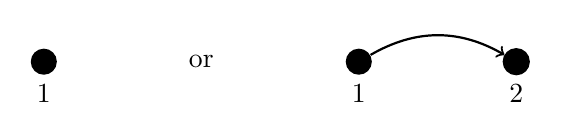
\begin{tikzpicture}
      \node[circle,fill,label={below:$1$}] (C) at (-1,0) {};
      \node at (1,0) {or};
      \node[circle,fill,label={below:$1$}] (A) at (3,0) {};
      \node[circle,fill,draw,label={below:$2$}] (B) at (5,0) {};
      \draw[->,thick] (A) to[bend left] (B);
    \end{tikzpicture}
    \item Compare: $\qt{\exists}{y}\qt{\forall}{x}\, A\qr{x}{y} \models \qt{\forall}{x}\exists
    y\,A\qr{x}{y}$!
    \item $\qt{\exists}{y}\qt{\forall}{x}\,(\lnot x=y \to
    A\qr{x}{y})$, $\qt{\forall}{x}\qt{\exists}{y}\,(\lnot x=y \land
    A\qr{x}{y})$ are jointly satisfiable.
    \item[]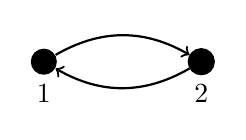
\begin{tikzpicture}
      \node[circle,fill,label={below:$1$}] (A) at (-1,0) {};
      \node[circle,fill,draw,label={below:$2$}] (B) at (1,0) {};
      \draw[->,thick] (A) to[bend left] (B);
      \draw[->,thick] (B) to[bend left] (A);
  \end{tikzpicture}
  \item $\qt{\forall}{x}\qt{\exists}{y}\,(\lnot x=y \land
  A\qr{x}{y}) \not\models \qt{\exists}{y}\qt{\forall}{x}\,(\lnot x=y \to
  A\qr{x}{y})$.
  \item[]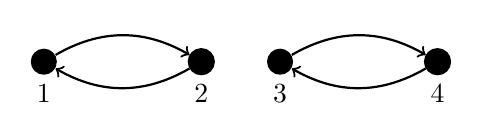
\begin{tikzpicture}
    \node[circle,fill,label={below:$1$}] (A) at (-1,0) {};
    \node[circle,fill,draw,label={below:$2$}] (B) at (1,0) {};
    \draw[->,thick] (A) to[bend left] (B);
    \draw[->,thick] (B) to[bend left] (A);
    \node[circle,fill,label={below:$3$}] (C) at (2,0) {};
    \node[circle,fill,draw,label={below:$4$}] (D) at (4,0) {};
    \draw[->,thick] (C) to[bend left] (D);
    \draw[->,thick] (D) to[bend left] (C);
\end{tikzpicture}
  \end{itemize}
\end{frame}

\subsection{Properties of relations}

\begin{frame}{Relations and extensions}
  
  \begin{itemize}[<+->]
    \item 2-place predicate symbols express relations.
    \item Extension of a 2-place predicate symbol is a set of ordered pairs.
    \item This is exactly how mathematicians think of relations.
    \item Let's think of properties relations can have, and categorize
    relations by these properties.
  \end{itemize}
\end{frame}

\begin{frame}{Reflexivity}
  \begin{definition}
    A relation $R$ is \emph{reflexive} if every object stands in the
    relation $R$ to itself.
  \end{definition}
\pause
  \begin{itemize}[<+->]
    \item $x$ is the same age as $y$.
    \item $x$ and $y$ share a parent.
    \item Not: $x$ and $y$ are siblings.
    \item $x \le y$ but not $x < y$.
    \item $x \mid y$ ($x$ divides $y$ without remainder) .
  \end{itemize}

  \begin{block}<7>{Expressing reflexivity in QL}
    The extension of $P$ in an interpretation is reflexive
    if and only if $\qt{\forall}{x}\,P\qr{x}{x}$ is true.
  \end{block}
\end{frame}


\begin{frame}{Symmetry}
  \begin{definition}
    A relation $R$ is \emph{symmetric} if whenever it holds in one
    direction, it also holds in the other.
  \end{definition}
\pause
  \begin{itemize}[<+->]
    \item $x$ is the same age as $y$.
    \item $x$ and $y$ share a parent.
    \item $x$ and $y$ are siblings.
    \item Not $x \le y$ or $x < y$.
    \item Not $x \mid y$.
  \end{itemize}

  \begin{block}<7>{Expressing symmetry in QL}
    The extension of $P$ in an interpretation is symmetric
    if and only if $\qt{\forall}{x}\qt{\forall}{y}(P\qr{x}{y} \to P\qr{y}{x})$ is true.
  \end{block}
\end{frame}


\begin{frame}{Transitivity}
  \begin{definition}
    A relation $R$ is \emph{transitive} if whenever it holds between
    $x$ and $y$ and $y$ and $z$, it also holds between $x$ and $z$.
  \end{definition}
\pause
  \begin{itemize}[<+->]
    \item $x$ is the same age as $y$.
    \item Not: $x$ and $y$ share a parent.
    \item Not: $x$ and $y$ are siblings.
    \item $x \le y$ and $x < y$.
    \item $x \mid y$.
  \end{itemize}

  \begin{block}<7>{Expressing transitivity in QL}
    The extension of $P$ in an interpretation is transitive
    if and only if $\qt{\forall}{x}\qt{\forall}{y}\qt{\forall}{z}((P\qr{x}{y} \land P\qr{y}{z} \to P\qr{x}{z})$ is true.
  \end{block}
\end{frame}

\begin{frame}{Anti-Symmetry}
  \begin{definition}
    A relation $R$ is \emph{anti-symmetric} if it never holds in both
    directions, except possibly for things being $R$-related to themselves.
  \end{definition}
\pause
  \begin{itemize}[<+->]
    \item Not: $x$ is the same age as $y$.
    \item Not: $x$ and $y$ share a parent.
    \item Not: $x$ and $y$ are siblings.
    \item $x \le y$.
    \item $x \mid y$ but only on the natural numbers!
  \end{itemize}

  \begin{block}<7>{Expressing anti-symmetry in QL}
    The extension of $P$ in an interpretation is anti-symmetric
    if and only if $\qt{\forall}{x}\qt{\forall}{y}((P\qr{x}{y} \land P\qr{y}{x}) \to x=y)$ is true.
  \end{block}
\end{frame}

\begin{frame}{QL and properties of relations}
  \begin{itemize}[<+->]
    \item A relation is \emph{universal} iff $\qt{\forall}{x}\qt{\forall}{y}\,P\qr{x}{y}$.
    \item Every universal relation is also:
    \begin{itemize}
      \item reflexive: $\qt{\forall}{x}\qt{\forall}{y}\,P\qr{x}{y} \models \qt{\forall}{x}\,P\qr{x}{x}$
      \item symmetric: $\qt{\forall}{x}\qt{\forall}{y}\,P\qr{x}{y} \models \forall
      x\qt{\forall}{y}(P\qr{x}{y} \to P\qr{y}{x})$
      \item transitive: $\qt{\forall}{x}\qt{\forall}{y}\,P\qr{x}{y} \models \forall
      x\qt{\forall}{y}\qt{\forall}{z}((P\qr{x}{y} \land P\qr{y}{z}) \to P\qr{x}{z})$.
    \end{itemize}
    \item But not vice versa!
  \end{itemize}
\end{frame}

\begin{frame}{QL and properties of relations}
  \begin{itemize}[<+->]
    \item Relations can be symmetric and anti-symmetric at the same time:
    \item The following are jointly satisfiable:
    \begin{align*}
      & \qt{\forall}{x}\qt{\forall}{y}(P\qr{x}{y} \to P\qr{y}{x})\\
      & \qt{\forall}{x}\qt{\forall}{y}((P\qr{x}{y} \land P\qr{y}{x}) \to x=y)
    \end{align*}
    \item Relations can be transitive and symmetric without being reflexive:
    \item We have:
    \begin{align*}
      & \qt{\forall}{x}\qt{\forall}{y}\qt{\forall}{z}((P\qr{x}{y} \land P\qr{y}{z} \to P\qr{x}{z})\\
      & \qt{\forall}{x}\qt{\forall}{y}(P\qr{x}{y} \to P\qr{y}{x})\\
      \not\models\quad & \qt{\forall}{x}\, P\qr{x}{x}
    \end{align*}
  \end{itemize}
\end{frame}